\documentclass[12pt,a4paper]{article}
\usepackage[utf8]{inputenc}%Para Tildes y ñ%
\usepackage[spanish]{babel}
\usepackage{amsmath}
\usepackage{amsfonts}
\usepackage{amssymb}
\usepackage{siunitx}
\usepackage{adjustbox}
%\usepackage{minted}
\usepackage[american]{circuitikz}
\usepackage{tikz}
\usepackage{graphicx} 
\usepackage{pdfpages} %para importar paginas de un pdf 
\usepackage{booktabs}
\usepackage{multicol}
\usepackage[bookmarks = true, colorlinks=true, linkcolor = black, citecolor = green, menucolor = black, urlcolor = black]{hyperref} 
\usepackage[left=2cm,right=2cm,top=2cm,bottom=2cm]{geometry} 
\usepackage{multirow}
\addto\captionsspanish{\renewcommand{\listtablename}{Índice de tablas}}		% Cambiar nombre a lista de tablas   
\addto\captionsspanish{\renewcommand{\tablename}{Tabla}}					% Cambiar nombre a tablas
\usepackage{float}		% Para ubicar las tablas y figuras justo después del texto
\usepackage{pdfpages}
\usepackage{enumerate}%listas y viñetas
\author{Estudiantes:\\ Kevin Campos Castro\\ Josué Salmerón Córdoba  \\{\small Grupo 1}\\ Profesor:  Marco Villalta  \vspace*{3.0in}}
\title{Universidad de Costa Rica\\{\small Facultad de Ingeniería\\Escuela de Ingeniería Eléctrica\\IE0624 – Laboratorio 4\\III ciclo 2023\\\vspace*{0.55in}}\\ Título: STM32: GPIO, ADC, comunicaciones, Iot. \vspace*{1.35in}}
%\date{fecha de entrega} 

\begin{document} 

\maketitle  
\thispagestyle{empty}%%no numerar la portada
\renewcommand{\thepage}{\roman{page}}
\newpage
\tableofcontents
\newpage
\listoffigures 
\newpage
\listoftables  
\newpage
%%%%%%%%%%  
\renewcommand{\thepage}{\arabic{page}} 
\setcounter{page}{1}
\begin{center}
\section{Resumen}
\end{center}
% AQUI VA EL RESUMEN 

%\textbf{\textit{Palabras clave}} \\

%palabras,clave,separadas, por,coma (solo en el reporte)
   
\newpage  


%\section{Objetivos}
\subsection{Objetivos General}
\begin{itemize}
\item obj gral. 

\end{itemize}

\subsection{Objetivos Específicos}
\begin{itemize}
\item objetivo 1
\item objetivo 2  

\end{itemize} 
\newpage
\section{Nota teórica}
En esta sección se describen los componentes principales que se utilizaron para el desarrollo de un sismógrafo.
\subsection*{STM32F429 Discovery kit}
Este microcontrolador permite a los usuarios desarrollar fácilmente aplicaciones de alto desempeño. Incluye un ST-LINK/V2 embebido como una herramienta de depuración, una SRAM externa de 64-Mbit, un ST MEMS giroscopio, un USB OTG conector AB, LEDs y botones. Algunas de las características generales se resumen a continuación.

\subsubsection*{Características generales}
Las características más importantes de este mcu se mencionan a continuación:
\begin{multicols}{2}
 \begin{itemize}
    \item 2.4 QVGA TFT LCD.
    \item 64-Mbit SDRAM.
    \item USB OTG con conector Micro-AB.
    \item Header para LQFP144 I/Os.
    \item Sensor de movimiento I3G4250D, Giroscopio ST MEMS de 3-ejes-
    \item On-board ST-LINK/V2-B.
    \item Alimentación por USB o fuente externa de \SI{3}{\volt} o \SI{5}{\volt}.
    \item 2  push-button (Usuario y reset).
    \item Core: ARM 32 bits Cortex-M4 con FPU (RISC).
    \item Debug: SWD, JTAG.
    \item Trabaja en frecuencia de \SI{180}{\mega\Hz}
    \item 168 I/O con capacidad de interrupción.
    \item 2MB flash, 256 KB SRAM.
    \item Controlador LCD-TFT.
    \item 21 interfaces de comunicaciones(I2C,USART,SPI,SAI,CAN).
    \item Low Power.
    \item Conectividad avanzada USB 2.0.
    \item Intefaz de camara.
    \item 2x12bit convertidor D/A.
    \item True RNG.
    \item CRC.
    \item 6 LEDS: LD1 (USB Comms), LD2(3.3V PowerOn, 2 LEDS de ususario (LD3 y LD4), 2 LEDS USB OTG (LD5 y LD6).
    \item Controladores DMA.
    \item 17 timers: 12 timers de 16bit, 2 de 32bit de hasta 180MHz, c/u con 4IC/OC/PWM.
\end{itemize}   
\end{multicols}

\subsubsection*{Diagrama de bloques}
En la figura \ref{fig1} se muestra el diagrama de bloques del STM32F429.
\begin{figure}[H]
\centering
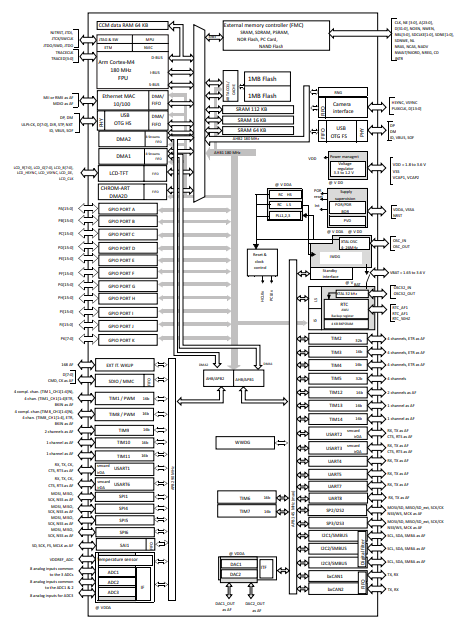
\includegraphics[width=.55\linewidth]{Imagenes/1.png}
 \caption{Diagrama de bloques del STM32F429 . Tomado de \cite{web}.}
 \label{fig1}
\end{figure}
\subsubsection*{Diagrama de pines}
Luego, el diagrama de pines de este mcu se presenta en la figura \ref{fig2}
\begin{figure}[H]
\centering
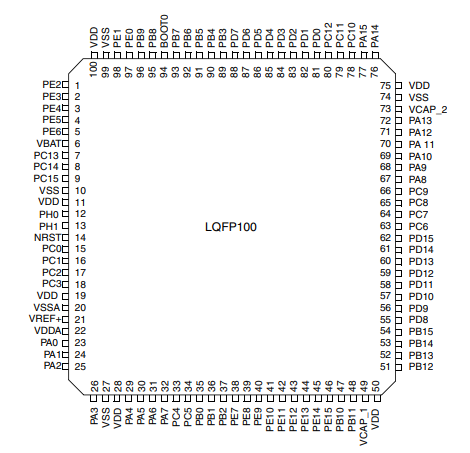
\includegraphics[width=.55\linewidth]{Imagenes/2.png}
 \caption{Diagrama de pines del STM32F429. Tomado de \cite{web}.}
 \label{fig2}
\end{figure}
\subsubsection*{Características eléctricas}
Las siguientes tablas resumen las características eléctricas de este microcontrolador.
\begin{figure}[H]
\centering
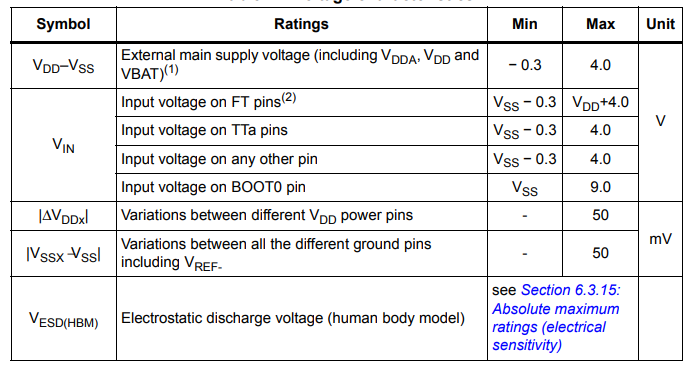
\includegraphics[width=.55\linewidth]{Imagenes/3.png}
 \caption{Detalles del voltaje del mcu. Tomado de \cite{web}.}
 \label{fig3}
\end{figure}

\begin{figure}[H]
\centering
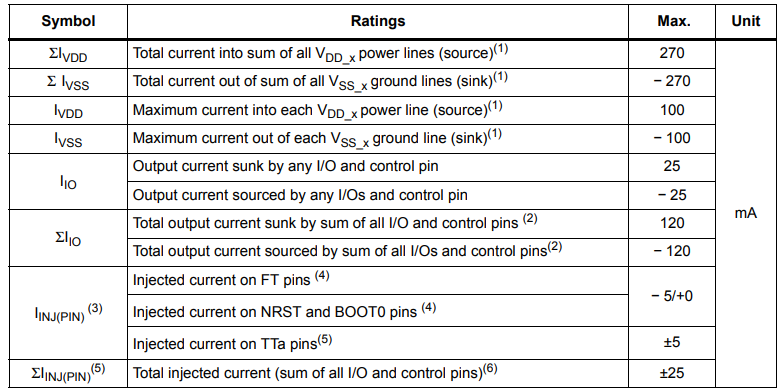
\includegraphics[width=.55\linewidth]{Imagenes/4.png}
 \caption{Detalles de la corriente en el mcu. Tomado de \cite{web}.}
 \label{fig4}
\end{figure}


\subsection*{Periféricos utilizados}
Los registros utilizados en este laboratorio se describen a continuación:
\begin{itemize}
    \item WHO\_AM\_I: Registro utilizado como identificador.
    \item CTRL\_REG1: Registro utilizado para habilitar registros de lectura de ejes.
    \begin{figure}[H]
        \centering
        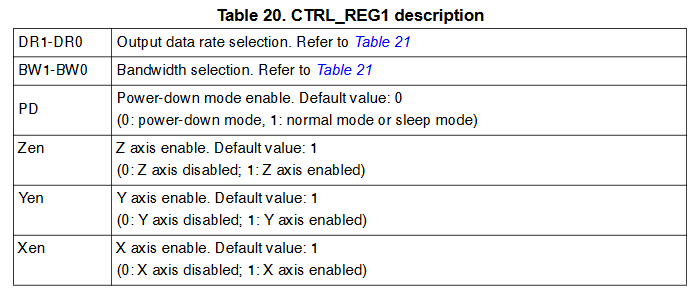
\includegraphics[width=.7\linewidth]{Imagenes/k1.png}
        \caption{Descripción del registro CTRL\_REG1. Tomado de \cite{l3gd20}.}
        \label{fig5}
    \end{figure}
    \item CTRL\_REG4: Este registro es utilizado para la configuración del DPS y también para la configuración del modo de selección del SPI.
    \begin{figure}[H]
        \centering
        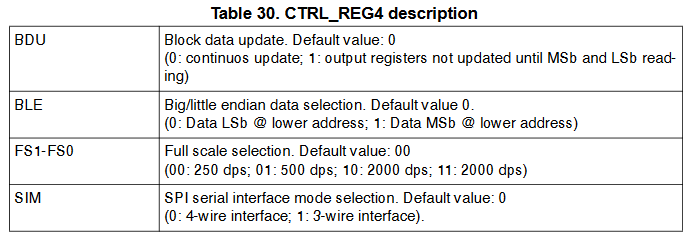
\includegraphics[width=.7\linewidth]{Imagenes/k2.png}
        \caption{Descripción del registro CTRL\_REG4. Tomado de \cite{l3gd20}.}
        \label{fig6}
    \end{figure}
    Para la lectura de los ejes, se utilizan los siguientes registros, ambos son registros de 8 bits. La \textbf{L} es para representar los primeros 8 bits menos significativos y la \textbf{H} para los 8 bits más significativos, ambos de la lectura del giroscopio en el eje indicado (X, Y o Z).
    \item OUT\_X\_L y OUT\_X\_H
    \item OUT\_Y\_L y OUT\_Y\_H
    \item OUT\_Z\_L y OUT\_Z\_H
    \item STATUS\_REG
    \begin{figure}[H]
        \centering
        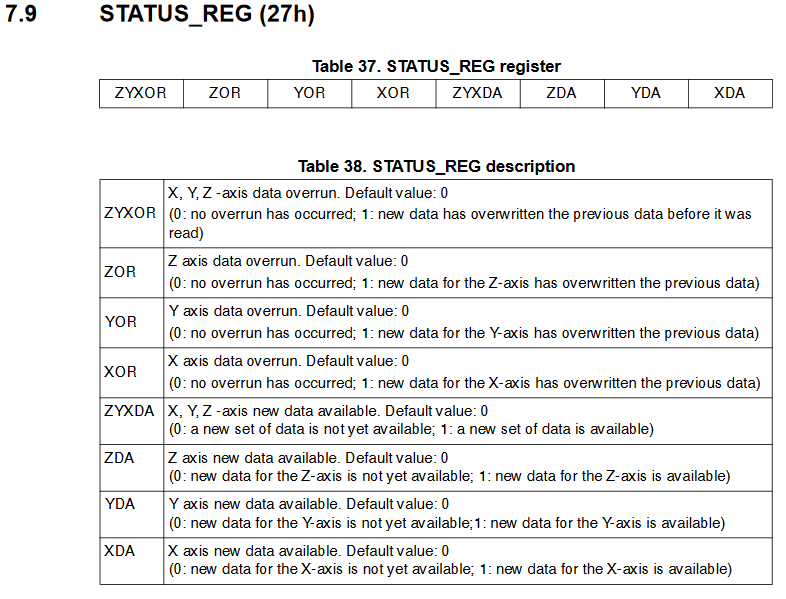
\includegraphics[width=.7\linewidth]{Imagenes/k3.png}
        \caption{Descripción del registro STATUS\_REG. Tomado de \cite{l3gd20}.}
        \label{fig7}
    \end{figure}
\end{itemize}

\subsection*{Componentes electrónicos complementarios}
% quiza mencionar la ayuda de la protoboard, en realidad fue como lo único.
Es un circuito que lo compone una electrónica básica (así lo resume la tabla \ref{table_2}), solo se usó una protoboard y 3 resistencias en total, una batería de \SI{9}{\volt}, esto para realizar un divisor de tensión con el objetivo de alimentar a la placa STM32249 Discovery Kit con \SI{5}{\volt}. Así, se sabe que $v_{out} \approx \SI{5}{\volt}$
\begin{itemize}
\item $R_1 = \SI{1}{\kilo\ohm}$
\item $R_2 = \SI{1.8}{\kilo\ohm}$
\item $v_{in} =  \SI{9}{\volt}$
\end{itemize}
Aplicando el divisor de tensión se tiene que:
\begin{equation}
v_{out} = \SI{9}{\volt} \cdot \frac{  \SI{1}{\kilo\ohm} }{ \SI{1}{\kilo\ohm}+\SI{1.8}{\kilo\ohm}} \approx \SI{3.21}{\volt}
\label{eq1}
\end{equation}
De la ecuación \ref{eq1}, se demuestra que con estas magnitudes es posible alimentar la placa sin sobrepasar el umbral.
\subsection*{Lista de componentes}
La lista de componentes fueron consultados en \cite{web2} disponibles
\begin{table}[H]
\caption{Lista de equipos}
\label{table_2}
\begin{center}
\begin{tabular}{r|cc}
\hline
\textbf{Componente}&\textbf{Cantidad}&\textbf{Precio}\\
 \hline
STM32F429 Discovery Kit& 1 & 83\$ \\ \hline 
Resistencias \SI{20}{\kilo\ohm}&2 & 0.4\$ \\ \hline 
Resistencias \SI{18}{\kilo\ohm}&1 & 0.2\$ \\ \hline 
Protoboard &1 &10\$ \\ \hline 
Broche porta pila &1 &0.5\$ \\ \hline 
Baterías \SI{9}{\volt} & 2& 2\$ \\ \hline 

 \textbf{Total}& & 96.1\$ \\
 \hline
\end{tabular}
\end{center}
\end{table}

\subsection*{Diseño del circuito}
El diagrama mostrado en la figura \ref{DF_S}, resume el funcionamiento del sismógrafo.
\begin{figure}
\centering


\tikzset{every picture/.style={line width=0.75pt}} %set default line width to 0.75pt        

\begin{tikzpicture}[x=0.75pt,y=0.75pt,yscale=-1,xscale=1]
%uncomment if require: \path (0,616); %set diagram left start at 0, and has height of 616

%Flowchart: Connector [id:dp7813495520702245] 
\draw   (315,40) .. controls (315,25.64) and (326.64,14) .. (341,14) .. controls (355.36,14) and (367,25.64) .. (367,40) .. controls (367,54.36) and (355.36,66) .. (341,66) .. controls (326.64,66) and (315,54.36) .. (315,40) -- cycle ;
%Straight Lines [id:da8847526091998554] 
\draw    (339.92,67) -- (339.92,83) ;
\draw [shift={(339.92,86)}, rotate = 270] [fill={rgb, 255:red, 0; green, 0; blue, 0 }  ][line width=0.08]  [draw opacity=0] (8.93,-4.29) -- (0,0) -- (8.93,4.29) -- cycle    ;
%Flowchart: Decision [id:dp21596588394867888] 
\draw   (335.35,181) -- (412,239.5) -- (335.35,298) -- (258.69,239.5) -- cycle ;
%Straight Lines [id:da7204417446380422] 
\draw    (335.35,162) -- (335.35,178) ;
\draw [shift={(335.35,181)}, rotate = 270] [fill={rgb, 255:red, 0; green, 0; blue, 0 }  ][line width=0.08]  [draw opacity=0] (8.93,-4.29) -- (0,0) -- (8.93,4.29) -- cycle    ;
%Straight Lines [id:da49582350632228556] 
\draw    (207.76,260) -- (207.76,276) ;
\draw [shift={(207.76,279)}, rotate = 270] [fill={rgb, 255:red, 0; green, 0; blue, 0 }  ][line width=0.08]  [draw opacity=0] (8.93,-4.29) -- (0,0) -- (8.93,4.29) -- cycle    ;
%Shape: Right Angle [id:dp2914826540765745] 
\draw   (258.69,239.5) -- (207.76,239.5) -- (207.76,260) ;
%Shape: Right Angle [id:dp7943090498770735] 
\draw   (333.35,580) -- (104,580) -- (104,72) ;
%Straight Lines [id:da15691850789793538] 
\draw    (332,353) -- (332.31,381) ;
\draw [shift={(332.35,384)}, rotate = 269.36] [fill={rgb, 255:red, 0; green, 0; blue, 0 }  ][line width=0.08]  [draw opacity=0] (8.93,-4.29) -- (0,0) -- (8.93,4.29) -- cycle    ;
%Flowchart: Process [id:dp025828036440153967] 
\draw   (157,279) -- (269,279) -- (269,331) -- (157,331) -- cycle ;
%Flowchart: Process [id:dp08317044111396199] 
\draw   (226,91) -- (429,91) -- (429,163) -- (226,163) -- cycle ;
%Flowchart: Decision [id:dp9588588712187942] 
\draw   (332.35,384) -- (409,442.5) -- (332.35,501) -- (255.69,442.5) -- cycle ;
%Straight Lines [id:da6075623967992321] 
\draw    (335.35,298) -- (335.35,314) ;
\draw [shift={(335.35,317)}, rotate = 270] [fill={rgb, 255:red, 0; green, 0; blue, 0 }  ][line width=0.08]  [draw opacity=0] (8.93,-4.29) -- (0,0) -- (8.93,4.29) -- cycle    ;
%Straight Lines [id:da7280821078053175] 
\draw    (204.76,463) -- (204.76,479) ;
\draw [shift={(204.76,482)}, rotate = 270] [fill={rgb, 255:red, 0; green, 0; blue, 0 }  ][line width=0.08]  [draw opacity=0] (8.93,-4.29) -- (0,0) -- (8.93,4.29) -- cycle    ;
%Shape: Right Angle [id:dp5301940302382446] 
\draw   (255.69,442.5) -- (204.76,442.5) -- (204.76,463) ;
%Flowchart: Process [id:dp03155186296961898] 
\draw   (156,482) -- (271,482) -- (271,509) -- (156,509) -- cycle ;
%Straight Lines [id:da1967066179049608] 
\draw    (333.35,561) -- (333.35,577) ;
\draw [shift={(333.35,580)}, rotate = 270] [fill={rgb, 255:red, 0; green, 0; blue, 0 }  ][line width=0.08]  [draw opacity=0] (8.93,-4.29) -- (0,0) -- (8.93,4.29) -- cycle    ;
%Flowchart: Process [id:dp5138152311739683] 
\draw   (277,319) -- (389,319) -- (389,349) -- (277,349) -- cycle ;
%Flowchart: Process [id:dp3581810005977748] 
\draw   (277,531) -- (389,531) -- (389,561) -- (277,561) -- cycle ;
%Straight Lines [id:da864404406808954] 
\draw    (332.35,501) -- (332.66,529) ;
\draw [shift={(332.69,532)}, rotate = 269.36] [fill={rgb, 255:red, 0; green, 0; blue, 0 }  ][line width=0.08]  [draw opacity=0] (8.93,-4.29) -- (0,0) -- (8.93,4.29) -- cycle    ;
%Straight Lines [id:da9757080202876469] 
\draw    (104,72) -- (336.92,72) ;
\draw [shift={(339.92,72)}, rotate = 180] [fill={rgb, 255:red, 0; green, 0; blue, 0 }  ][line width=0.08]  [draw opacity=0] (8.93,-4.29) -- (0,0) -- (8.93,4.29) -- cycle    ;

% Text Node
\draw (324,30) node [anchor=north west][inner sep=0.75pt]   [align=left] {Inicio};
% Text Node
\draw (299,220) node [anchor=north west][inner sep=0.75pt]   [align=left] {EnviaDatos\\==1};
% Text Node
\draw (302,295) node [anchor=north west][inner sep=0.75pt]   [align=left] {No};
% Text Node
\draw (199,220) node [anchor=north west][inner sep=0.75pt]   [align=left] {Si};
% Text Node
\draw (171,284) node [anchor=north west][inner sep=0.75pt]   [align=left] {Enviar datos\\LED\_1 = ON};
% Text Node
\draw (268,95) node [anchor=north west][inner sep=0.75pt]   [align=left] {Muestra giroscopio,\\estado batería,\\info pantalla};
% Text Node
\draw (302,428) node [anchor=north west][inner sep=0.75pt]   [align=left] {$\displaystyle 7\geqslant $batt};
% Text Node
\draw (198,423) node [anchor=north west][inner sep=0.75pt]   [align=left] {Si};
% Text Node
\draw (167,487) node [anchor=north west][inner sep=0.75pt]   [align=left] {LED\_2 = ON};
% Text Node
\draw (309,500) node [anchor=north west][inner sep=0.75pt]   [align=left] {No};
% Text Node
\draw (286,326) node [anchor=north west][inner sep=0.75pt]   [align=left] {LED\_1 = OFF};
% Text Node
\draw (279,536) node [anchor=north west][inner sep=0.75pt]   [align=left] {alarm\_LED= 0};


\end{tikzpicture}
\caption{Diagrama de flujo del circuito.}
\label{DF_S}
\end{figure}
En la siguiente sección se mostrará paso a paso su respectivo funcionamiento.
\newpage


\section{Desarrollo/Análisis}

Inicialmente se hizo la prueba del giroscopio para determinar que los 3 ejes funcionaran correctamente a la hora de mover la placa.
\begin{figure}[H]
\centering
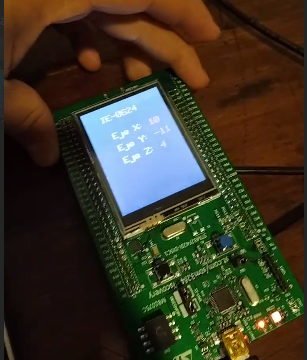
\includegraphics[width=.55\linewidth]{Imagenes/5.png}
 \caption{Funcionamiento del giroscopio.}
 \label{fig_gyro}
\end{figure}
Lo anterior se logró gracias los ejemplos dados de la biblioteca libopencm3. Y realizando otro tipo de depuraciones para darle un estilo a la presentación en la pantalla LCD.\par
Lo siguiente que se hizo fue la configuración de los GPIO's y establecer el pin \texttt{PA0} como entrada analógico y poder mostrar la tensión que posee la batería en el momento que es conectada. Inicialmente se hizo un divisor de tensión a partir de $v_{in}=\SI{9}{\volt}$, junto con resistencias de \SI{1.8}{\kilo\ohm} y \SI{1}{\kilo\ohm}, obtiendo una tensión de \SI{3.2}{\volt} tal como se muestra a continuación.
\begin{figure}[H]
\centering
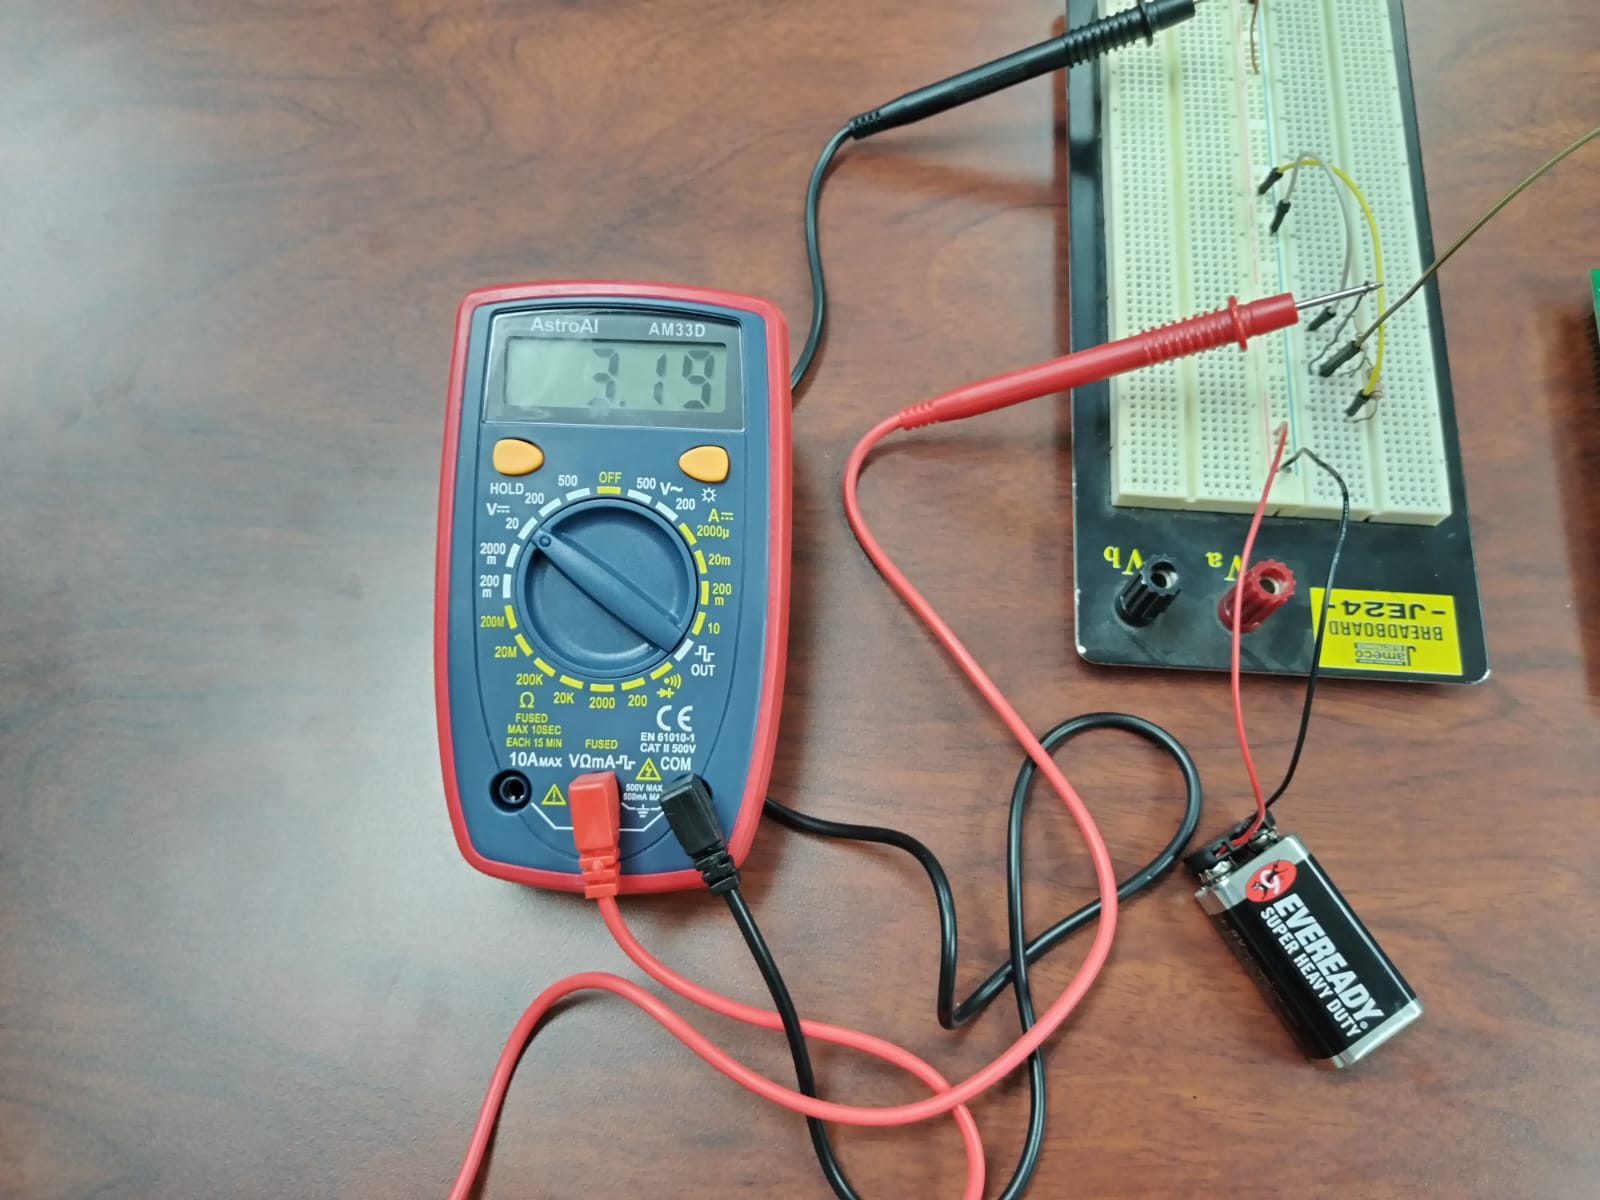
\includegraphics[width=.55\linewidth]{Imagenes/6.jpeg}
 \caption{Tensión de salida}
 \label{fig_vout}
\end{figure}
Esta tensión eléctrica es la que recibirá la placa por medio del pin \texttt{PA0}.
\begin{figure}[H]
\centering
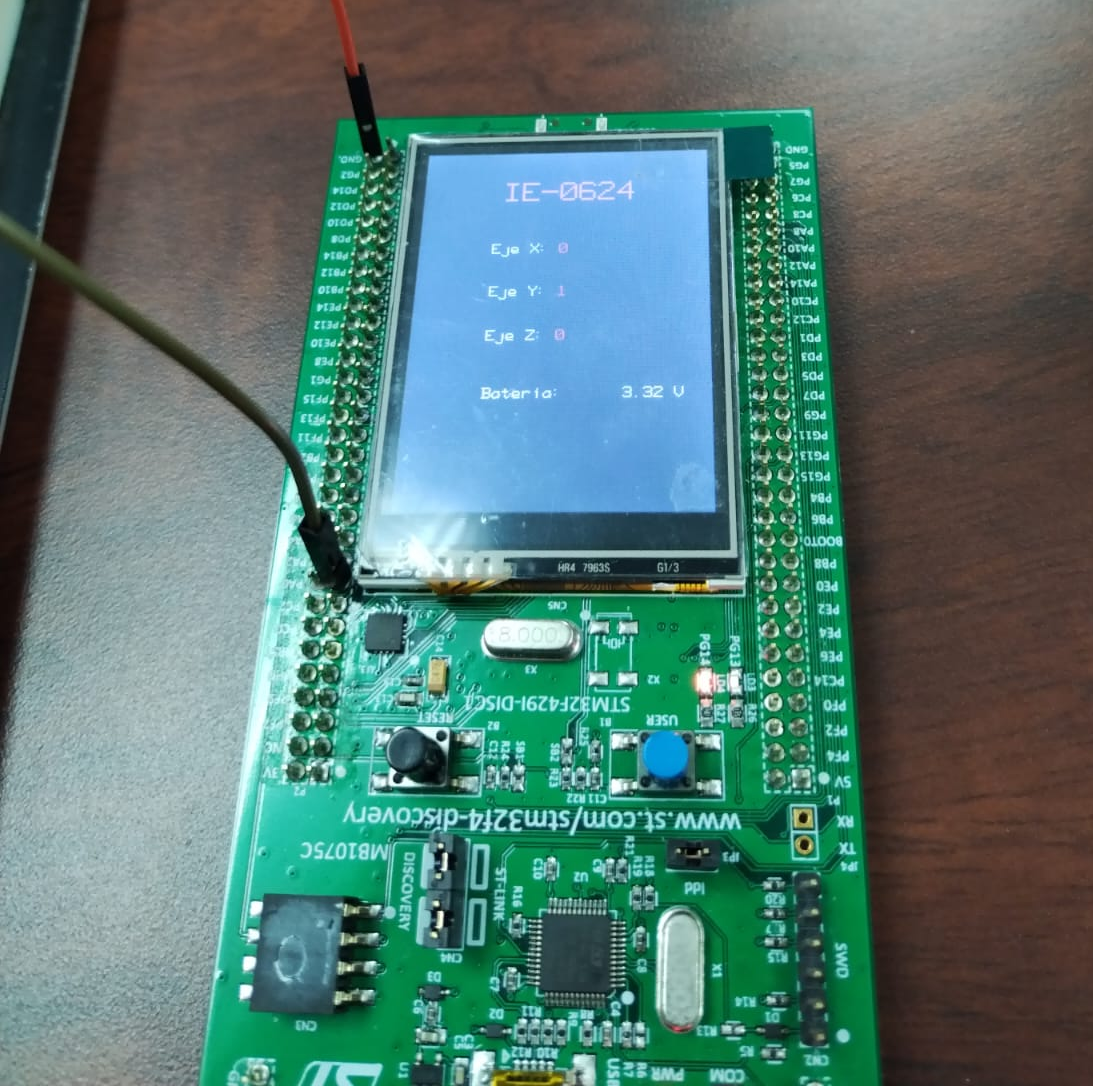
\includegraphics[width=.55\linewidth]{Imagenes/7.png}
 \caption{Magnitud de la batería menor a \SI{7}{\volt}.}
 \label{fig_bat}
\end{figure}
Además, note que de la figura anterior se muestra un LED encendido, lo cual indica una alarma ya que su valor es menor de \SI{7}{\volt}, sino fuera así, entonces el LED no debe encenderse.
\begin{figure}[H]
\centering
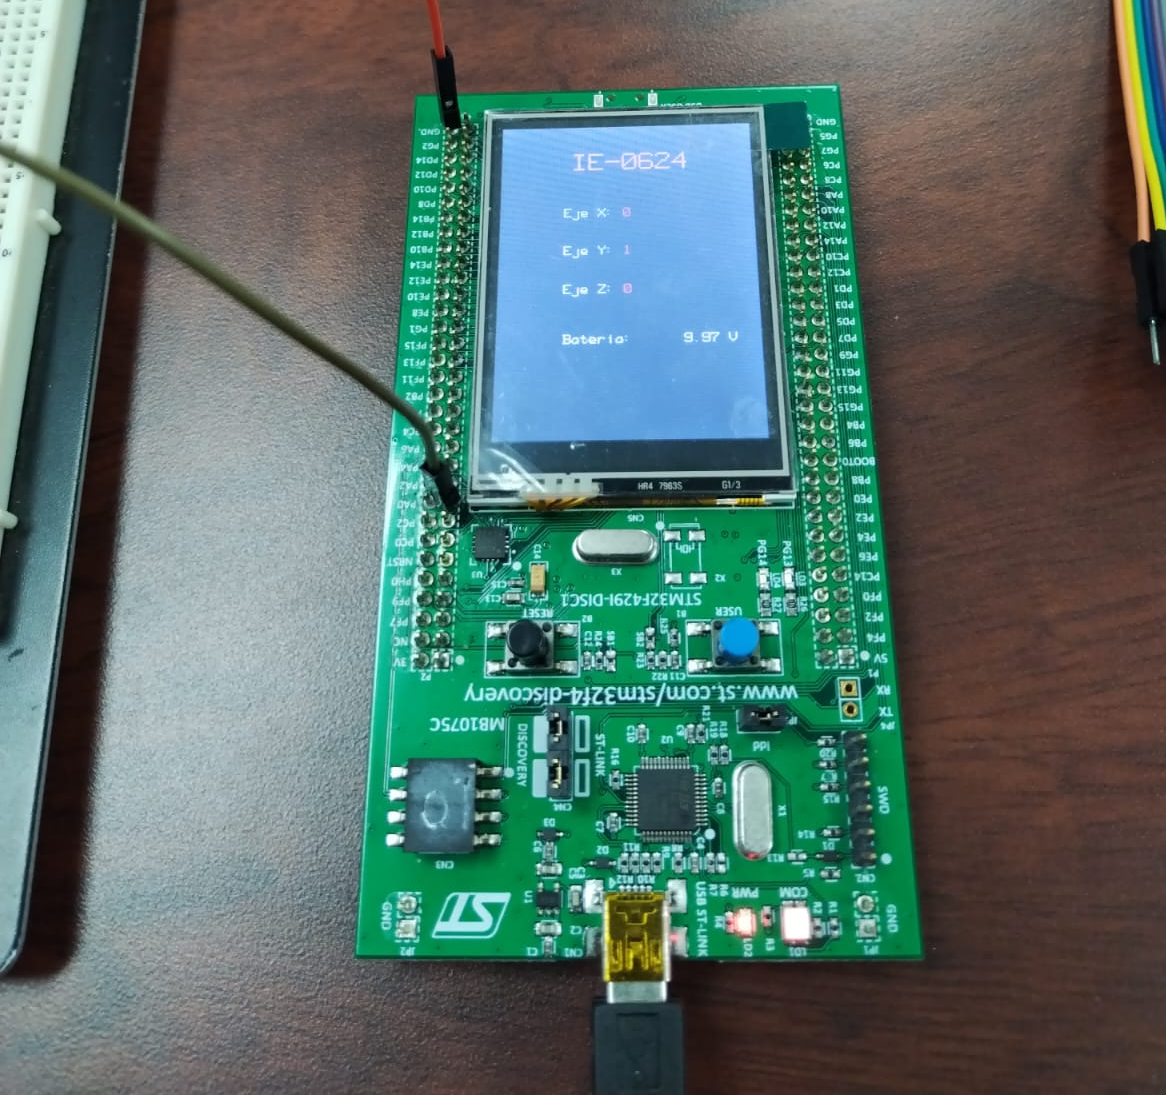
\includegraphics[width=.55\linewidth]{Imagenes/8.png}
 \caption{Magnitud de la batería mayor a \SI{7}{\volt}.}
 \label{fig_bat_OFF}
\end{figure}
Note que el LED \texttt{PG14} no se enciende, lo cual esta correctamente realizado.

\newpage
\section{Conclusiones y recomendaciones}
A partir de este trabajo se obtienen las siguientes conclusiones.
\begin{itemize}
\item El uso de los ejemplos brindados por la biblioteca \texttt{libopencm3} sirvió de ayuda para realizar las funciones del sismografo, ya que se logró ver elementos en la pantalla LCD, y a partir de esto se usaron los bloques de código necesarios para mostrar un simple texto, añadirle color, posición y otros detalles, ya con esto fue un gran avance y poder implementar el giroscopio con base a las demás configuraciones de \texttt{gpio} y sensibilidad en los ejes para mostrar los valores en cada eje.
\item Se aprendió como implementar una comunicación entre una nube y un microcontrolador.
\item A pesar de que no se lograron todos los puntos estipulados por el enunciado, se considera de que se lograron los más importantes. 
\item A partir de la tensión de salida en la batería (\SI{3.21}{\volt}) y haber realizado ajustes en funciones como \texttt{read\_adc\_naiive} se logró mostrar esta tensión en la pantalla y encender o apagar el LED respetando el umbral previamente dado.
\end{itemize}

Las recomendaciones de este trabajo son las siguientes:
\begin{itemize}
\item Verificar de que los datos se estén enviando de acuerdo al protocolo, varias veces se tuvieron problemas de que los datos no eran compatibles y esto era porque se le estaban enviando strings o ints y se esperaban bytes. El cálculo de un tiempo adecuado para que se dé la comunicación es muy importante y fue uno de los problemas más grandes que se tuvo con este laboratorio. La lectura de los ejemplos proporcionado fue de suma importancia para poder completar el laboratorio.
\item Probar los ejemplos que vienen en la librería \texttt{libopencm3}, esto ayuda a entender la funcionalidad de los bloques de código.
\item Realizar muchas pruebas y error con los ejemplos.
\item Crear el proyecto en la misma carpeta donde están los ejemplos, esto para no tener ningún problema a la hora de usar el makefile.
\item Tener mucho cuidado en las conexiones para cuidar el equipo de trabajo.
\end{itemize}



\newpage 

\bibliographystyle{unsrt}
\bibliography{bibliografia.bib}
\newpage

  \section{Anexos}
A continuación, se muestran las hojas del fabricante de los componentes usados para este laboratorio. 

%\includepdf[pages=1-14]{./Documentos/A000066-datasheet.pdf}
\foreach \page in {1, 20, 21,22, 35, 36, 43,45, 53-70, 93,94}{
  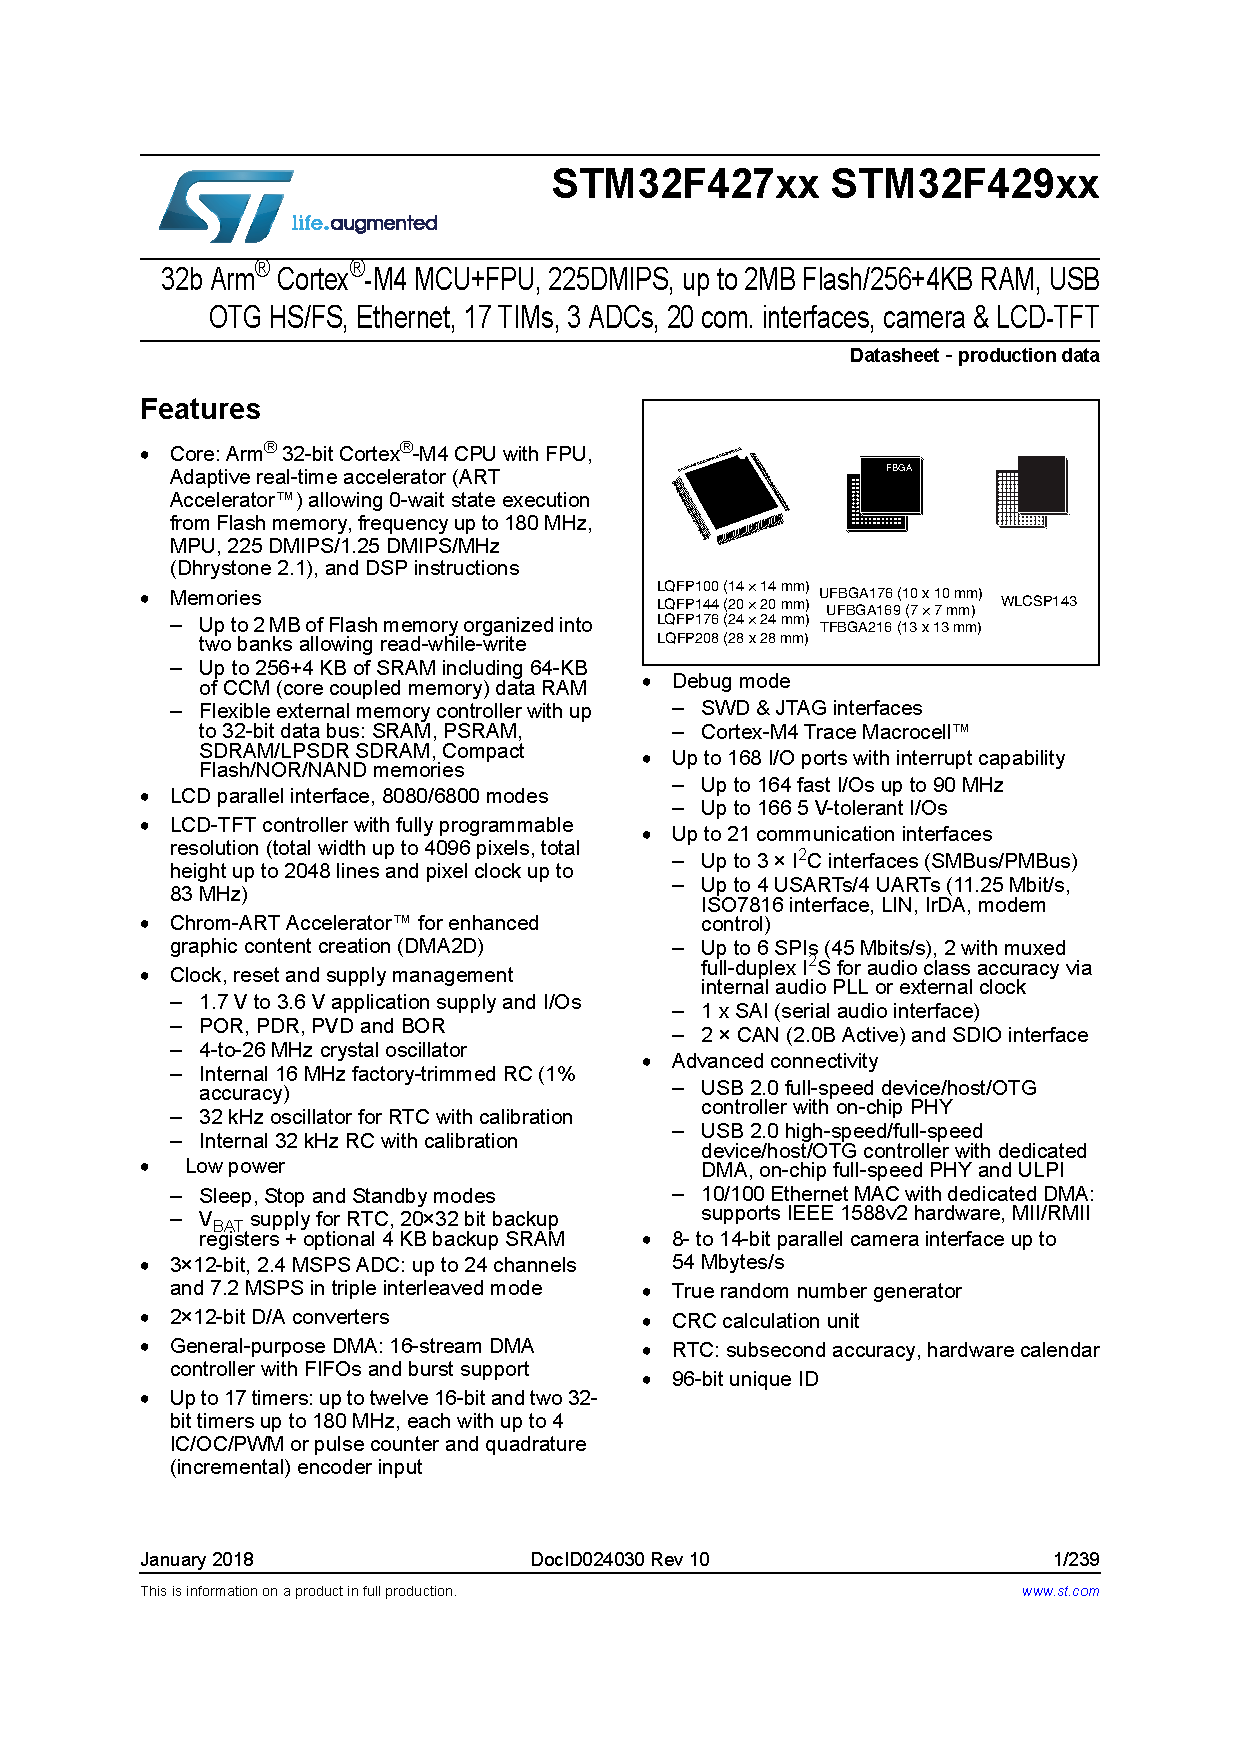
\includepdf[pages=\page]{./Documentos/stm32f429zi.pdf}
}
\foreach \page in {1, 15}{
  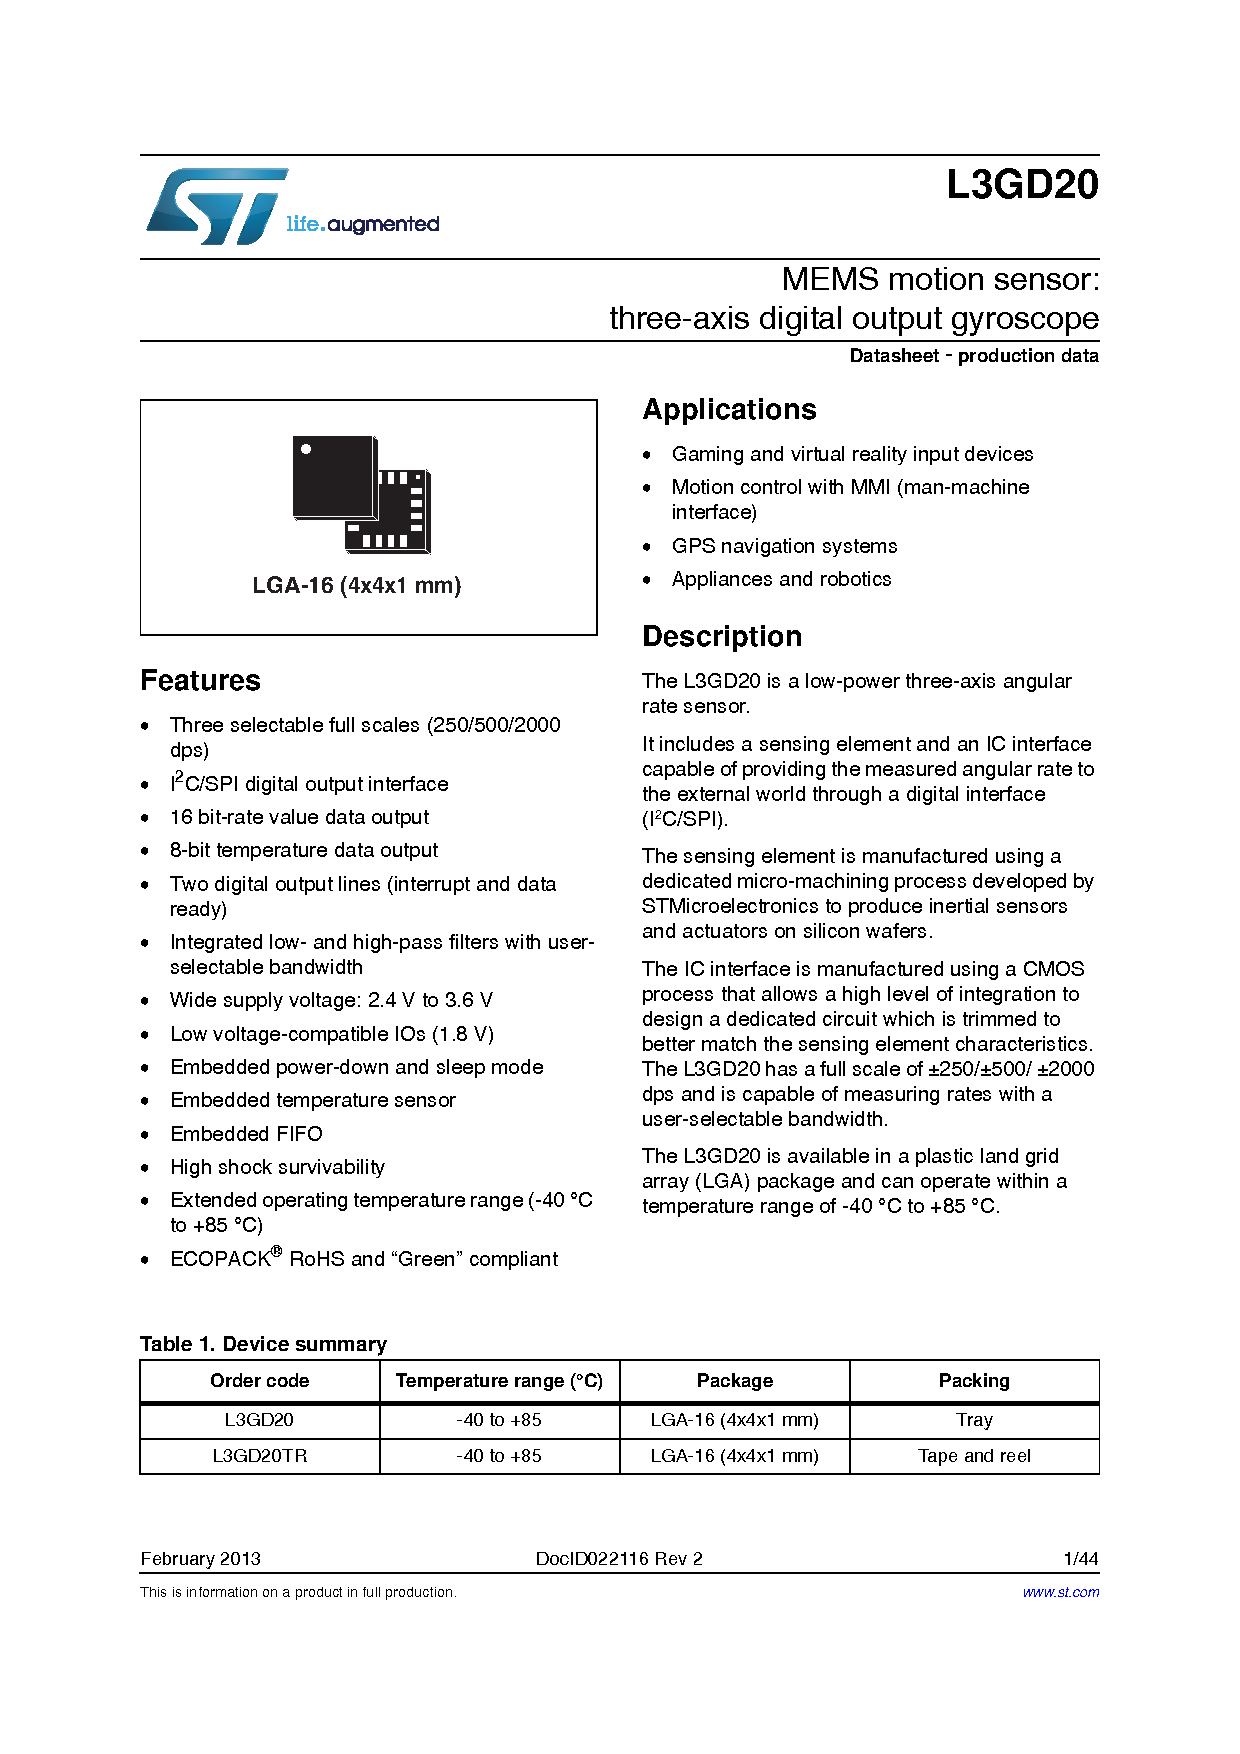
\includepdf[pages=\page]{./Documentos/l3gd20.pdf}
}
\foreach \page in {7}{
  
\includepdf[pages=\page]{./Documentos/ILI9341.pdf}
}
\end{document}
 

\end{document}